
\subsection{Overview and class diagram}
\label{sec:overview}


\begin{figure}[hbt]
\centering
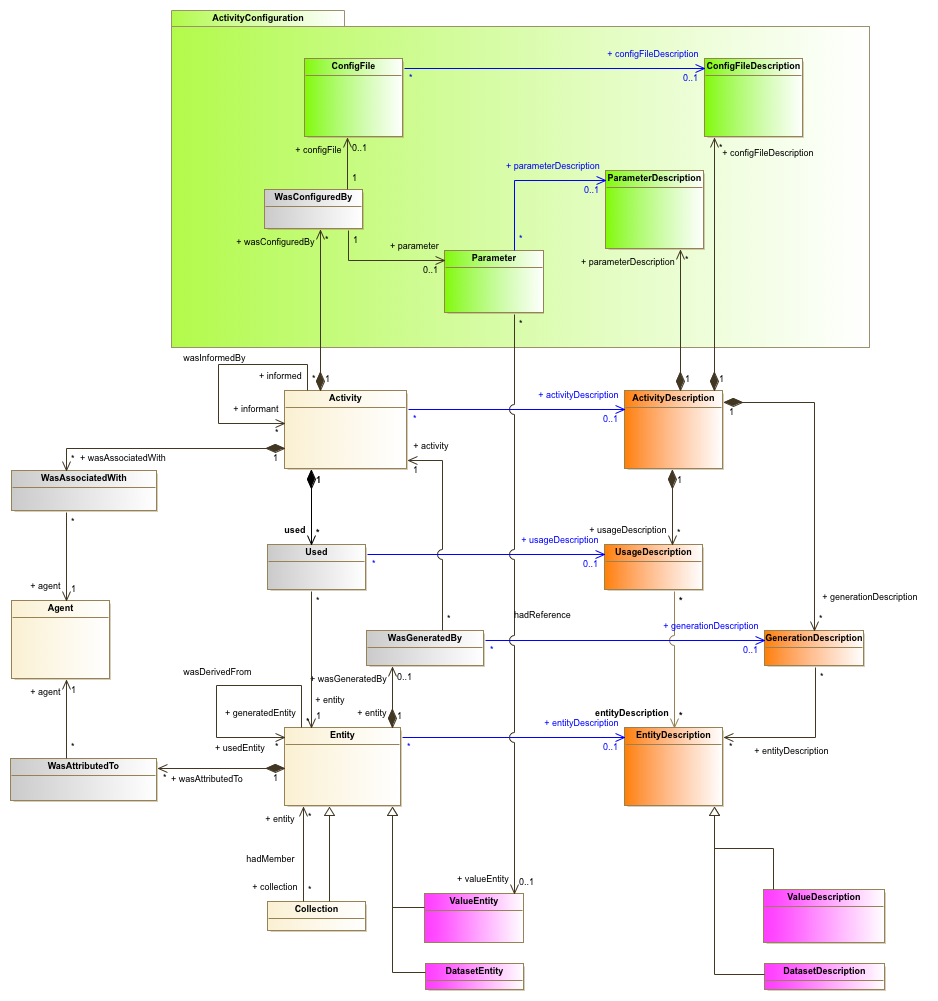
\includegraphics[width=1.0\textwidth]{PROV_Fig3.png}
\caption[Overview class diagram of the IVOA Provenance Data Model]{Overview class diagram of the IVOA Provenance Data Model. The core part in yellow is based on W3C PROV definitions where relations are shown in grey. It is extended by a description part (orange), specific types of entities (red) and an \class{ActivityConfiguration} package (green). A full diagram with attributes is shown in Section~\ref{sec:fulldiagram}, Figure~\ref{fig:fulldiagram}}
\label{fig:overview}
\end{figure}

The IVOA Provenance DM is based on the the PROV-DM recommendation \citep{std:W3CProvDM} of the World Wide Web Consortium (W3C), that provides the core elements of the model (see Sections~\ref{sec:ent_act} to~\ref{sec:agent+relations}). 
In the VO context, the provenance of something is thus a sequence of activities using and generating entities run by agents.

The model also includes description classes (see Section~\ref{sec:descriptions}) to provide information common to several elements; Specific types of \class{Entity} classes commonly used in astronomy (see Section~\ref{sec:spec_entities}); and an \class{ActivityConfiguration} package (see Section~\ref{sec:configuration}).

The IVOA Provenance DM is a class data model that follows the VO-DML designing rules \citep{2018ivoa.spec.0910L}. It is represented as a UML class diagram: an overview diagram is shown in Figure~\ref{fig:overview}, and a full diagram with attributes is shown in Appendix~\ref{sec:fulldiagram}, Figure~\ref{fig:fulldiagram}.


\subsection{Entity and Activity classes}
\label{sec:ent_act}

The core classes and relations of the IVOA Provenance DM are presented in Figure~\ref{fig:coreclasses}.
Traceability (see goal A in Section~\ref{sec:goals}) is enabled by chaining entities and activities, which are the building blocks of the history graph.


\begin{figure}[ht]
\centering
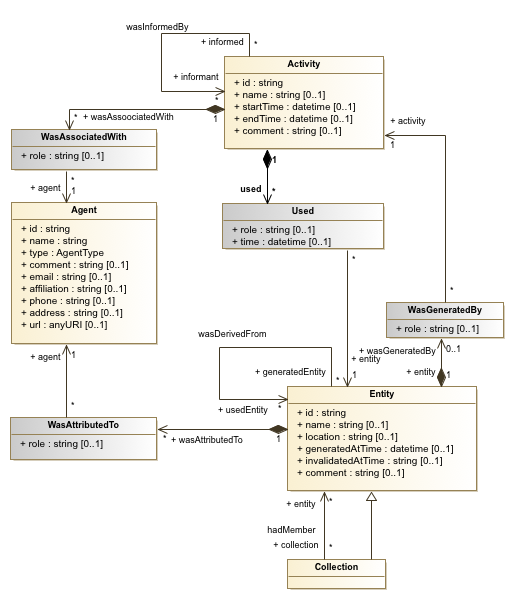
\includegraphics[width=1.0\textwidth]{PROV_Fig4.png}
\caption[Core classes and relations]{Core classes and relations. Attributes for these classes are detailed in tables found in Sections~\ref{sec:ent_act} to~\ref{sec:agent+relations}.}
\label{fig:coreclasses}
\end{figure}



\subsubsection{Entity and Collection classes}
\label{sec:Entity}

An \textbf{entity} is a physical, digital, conceptual, or other kind of thing with some fixed aspects (W3C PROV-DM \href{https://www.w3.org/TR/prov-dm/#term-entity}{\S5.1.1}). 

The \class{Entity} class in the model has the attributes given in Table \ref{tab:entity}.

Entities in astronomy are usually astronomical or astrophysical datasets in the form of images, tables, numbers, etc. But they can also be log files, files containing system information, any input or output value, environment variables, ambient conditions, or, in a wider sense, observation proposals, scientific articles, or manuals and other documents. 
Though the focus is on digital entities in this document, entities can also refer to physical entities that may be linked to digital entities, such as e.g., tools, instruments, detectors, photographic plates.


\begin{table}[ht]
\small
\tymax  0.5\textwidth
\textbf{\normalsize Entity}\vspace{0.25em}\\
\begin{tabulary}{1.0\textwidth}{llL}
\toprule
\head{Attribute} & \head{Data type} & \head{Description}\\
\midrule
\textbf{id} & string & a unique identifier for this entity\\
name        & string & a human-readable name for the entity\\
location    & string & a path or spatial coordinates, e.g., a URL/URI, latitude-longitude coordinates on Earth, the name of a place.\\
generatedAtTime  & datetime & date and time at which the entity was created (e.g., timestamp of a file)\\
invalidatedAtTime  & datetime & date and time of invalidation of the entity. After that date, the entity is no longer available for any use.\\
comment  &  string & text containing specific comments on the entity\\
\bottomrule
\end{tabulary}
\caption[Attributes of the \class{Entity} class]{Attributes of the \class{Entity} class. Attributes in \textbf{bold} are mandatory and must not be null.
}\label{tab:entity}
\end{table}


A \textbf{collection} is an entity that provides a structure to some constituents that must themselves be entities (W3C PROV-DM \href{https://www.w3.org/TR/prov-dm/#term-collection}{\S5.6.1}). These constituents are said to be members of the collections. They are connected in the model with a \class{hadMember} relation.


\subsubsection{Activity class}
\label{sec:activity}

An \textbf{activity} is something that occurs over a period of time and acts upon or with entities; it may include consuming, processing, transforming, modifying, relocating, using, or generating entities (W3C PROV-DM \href{https://www.w3.org/TR/prov-dm/#term-Activity}{\S5.1.2}). 

The \class{Activity} class in the model has the attributes given in Table \ref{tab:activity}.

Activities in astronomy include all steps from obtaining data to the reduction
of  images and production of new datasets, such as image calibration, bias
subtraction, image stacking, light curve generation from a number of
observations, radial velocity determination from spectra, post-processing steps
of simulations, etc.


\begin{table}[ht]
\small
\tymax  0.5\textwidth
\textbf{\normalsize Activity}\vspace{0.25em}\\
\begin{tabulary}{1.0\textwidth}{llL}
\toprule
\head{Attribute}  & \head{Data type} & \head{Description}\\
\midrule
\textbf{id}  & string & a unique id for this activity\\
name         & string & a human-readable name (to be displayed by clients)\\
startTime    & datetime & start of an activity\\
endTime      & datetime & end of an activity\\
comment      & string & text containing specific comments on the activity\\
\bottomrule
\end{tabulary}
\caption[Attributes of the \class{Activity} class.]{Attributes of the \class{Activity} class. Attributes in \textbf{bold} are mandatory and must not be null.}\label{tab:activity}
%, references are indicated with an arrow ($\rightarrow$).}
\end{table}


\subsection{Entity-Activity relations}
\label{sec:entity-activity-relations}

Each entity is usually a result of an activity, expressed by a link from the entity to its generating activity, and can be used as input for (many) other activities.
Thus the information on whether data are used as input or were produced as output of some activity is given by the \emph{relations} between activities and entities.
Tracking those relations answers one of the main objectives of the model (see goal A in Section~\ref{sec:goals}).


\subsubsection{Used class}

\textbf{Usage} is the beginning of utilizing an entity by an activity. Before usage, the activity had not begun to utilize this entity and could not have been affected by the entity (W3C PROV-DM \href{https://www.w3.org/TR/prov-dm/#term-Usage}{\S5.1.4}).

Usage is implemented in the model by a class \class{Used} that connects \class{Activity} to \class{Entity} and contains the attributes in Table~\ref{tab:used}.

For example, an activity ``calibration'' used entities with the roles ``calibration data'' and ``raw images''.

\begin{table}[ht]
\small
\tymax  0.5\textwidth
\textbf{\normalsize Used}\vspace{0.25em}\\
\begin{tabulary}{1.0\textwidth}{llL}
\toprule
\head{Attribute} & \head{Data type} & \head{Description}\\
\midrule
role  & string   & function of the entity with respect to the activity\\
time  & datetime & time at which the usage of an entity started\\
\bottomrule
\end{tabulary}
\caption[Attributes of the \class{Used} relation class]{Attributes of the \class{Used} relation class.}
\label{tab:used}
\end{table}

The \attribute{time} of the usage can be specified, and must be between the \attribute{startTime} and the \attribute{endTime} of the corresponding activity.

The \class{Used} class is closely coupled to the \class{Activity} by a composition (see \ref{sect:Composition}). 
Any given entity can be used by more than one activity.


\subsubsection{WasGeneratedBy class}

\textbf{Generation} is the completion of production of a new entity by an activity. This entity did not exist before generation and becomes available for usage after this generation (W3C PROV-DM \href{https://www.w3.org/TR/prov-dm/#term-Generation}{\S5.1.3}).
        
Generation is implemented in the model by a class \class{WasGeneratedBy} that connects \class{Entity} to \class{Activity} and contains the attributes in Table~\ref{tab:wasgeneratedby}.

For example, the entity ``raw\_image.fits'' was generated by the activity ``observation'' with the role ``raw image''.

\begin{table}[ht]
\small
\tymax  0.5\textwidth
\textbf{\normalsize WasGeneratedBy}\vspace{0.25em}\\
\begin{tabulary}{1.0\textwidth}{llL}
\toprule
\head{Attribute} & \head{Data type} & \head{Description}\\
\midrule
role   &  string   &  function of the entity with respect to the activity\\
%time & prov:time & datetime & time at which the generation of an entity is finished\\
\bottomrule
\end{tabulary}
\caption[Attributes of the \class{WasGeneratedBy} relation class]{Attributes of the \class{WasGeneratedBy} relation class.}
\label{tab:wasgeneratedby}
\end{table}

As the \class{Entity} class has an attribute \attribute{generatedAtTime}, there is no additional time attribute in this relation.

The \class{WasGeneratedBy} relation is closely coupled with the \class{Entity} via a composition (see \ref{sect:Composition}). 
An entity can be generated by only one activity, so the multiplicity is 1 or 0 between \class{Entity} and \class{WasGeneratedBy}.


\subsubsection{Roles in Entity-Activity relations}
\label{sec:roles}

The \attribute{role} of an entity within an activity should be provided.
Roles in \class{Entity}-\class{Activity} relations are free text attributes.

The \attribute{role} cannot be an attribute of the \class{Entity} class, since the same entity (e.g., a specific file containing an image) may play different roles with different activities.

In some cases the role is mandatory to distinguish two input entities. For example, an activity for dark-frame subtraction requires two input images. But it is very important to know which of the images is the raw image and which one fulfils the role of dark-frame.

Several entities may play the same role for an activity. For example, many image entities may be used as science-ready images for an image stacking process.



\subsubsection{WasDerivedFrom relation}

A \textbf{derivation} is a transformation of an entity into another, an update of an entity resulting in a new one, or the construction of a new entity based on a pre-existing entity (W3C PROV-DM \href{https://www.w3.org/TR/prov-dm/#term-Derivation}{\S5.2.1}).

Derivation is a relation \class{wasDerivedFrom} in the model, that connects an instance of \class{Entity} to another instance.

For example, the entity ``calibrated\_image.fits'' was derived from the entity ``raw\_image.fits''

This relation makes it possible to visualize independently the flow of entities, e.g., a dataflow. It does not need a priori a specific class or table in an implementation, but it provides a way to expose partial information that follows the general chain \class{WasGeneratedBy}-\class{Activity}-\class{Used} where the activity may be an empty instance because it is unknown or irrelevant.


\subsubsection{WasInformedBy relation}

\textbf{Communication} is the exchange of information (some unspecified entity) by two activities, one activity using some entity generated by the other (W3C PROV-DM \href{https://www.w3.org/TR/prov-dm/#term-Communication}{\S5.1.5}).

Communication is a relation \class{wasInformedBy} in the model, that connects an instance of \class{Activity} to another instance.

For example, the activity ``calibration'' was informed by the activity ``pipeline''.

This relation makes it possible to visualize independently the flow of activities as they occurred, which may be the result of the execution of a workflow. It does not need a priori a specific class or table in an implementation, but it provides a way to expose partial information that follows the general chain \class{Used}-\class{Entity}-\class{WasGeneratedBy} where the entity may be an empty instance because it is unknown or irrelevant.


\subsection{Agent and relations to Agent}
\label{sec:agent+relations}

A contact information is needed in case more information about a certain activity or entity is required, but also in order to know who was involved and to fulfil the Acknowledgement objective (see goal B in Section~\ref{sec:goals}).


\subsubsection{Agent class}
\label{sec:agent}

An \textbf{agent} is something that bears some form of responsibility for an activity taking place or for the existence of an entity (W3C PROV-DM \href{https://www.w3.org/TR/prov-dm/#term-agent}{\S5.3.1}).

The \class{Agent} class in the model has the attributes given in Table \ref{tab:agent}. 

An Agent is generally someone who pressed a button, ran a script, performed the observation or published a dataset. The agent can be a single person, a group of persons, a project or an institute (the vocabulary for agent types is given in Table~\ref{tab:agent-types}).

It is recommended to use organizational agents and agents with generic contacts.


\begin{table}[ht]
\small
\tymax  0.5\textwidth
\textbf{\normalsize Agent}\vspace{0.25em}\\
\begin{tabulary}{1.0\textwidth}{llL}
\toprule
\head{Attribute} & \head{Data type} & \head{Description}\\
\midrule
\textbf{id}    & string & unique identifier for an agent\\
\textbf{name}  & string & a common name for this agent; e.g., first name and last name; project name,  pipeline team, data center.\\
type        & AgentType & type of the agent as given in Table~\ref{tab:agent-types}\\
comment     & string & text containing specific comments on the agent\\
email       & string & contact email of the agent\\
affiliation & string & affiliation of the agent\\
phone       & string & phone number\\
address     & string & address of the agent\\
url         & anyURI & reference URL to the agent\\
\bottomrule
\end{tabulary}
\caption[Attributes of the \class{Agent} class]{Attributes of the \class{Agent} class. Attributes in \textbf{bold} are mandatory and must not be null.}
\label{tab:agent}
\end{table}

\begin{table}[ht]
\small
\tymax  0.5\textwidth
\textbf{\normalsize AgentType}\vspace{0.25em}\\
\begin{tabulary}{1.0\textwidth}{lp{8cm}}
\toprule
\head{Type} &\head{Description} \\
\midrule
Person        & person agents are people\\
Organization  & a social or legal institution, e.g., an institute, a consortium, a project\\
SoftwareAgent & running software, e.g., a cron job or a trigger \\
\bottomrule
\end{tabulary}
\caption[Enumeration of Agent types.]{Enumeration of Agent types.}
\label{tab:agent-types}
\end{table}

% 2018-12 commented
%A definition of organizations is given in the 
%IVOA Recommendation on Resource Metadata \citep{std:ResourceMeta}, hereafter 
%referred to as RM: ``An organization is [a] specific type of resource that 
%brings people together to pursue participation in VO applications.''
%It also specifies further that scientific projects can be considered 
%as organizations on a finer level:
%``At a high level, an organization could be a university, observatory, or government
%agency. At a finer level, it could be a specific scientific project, space mission,
%or individual researcher. A provider is an organization that makes data and/or services
%available to users over the network.''

For each agent a \attribute{name} must be specified. 
Other attributes can help locate or contact the agent (\attribute{email}, \attribute{affiliation}, \attribute{phone}, \attribute{address}).
Not every project will need them; e.g. an advanced system may use permanent identifiers (ORCIDs, identities in federations, etc) to identify agents, and retrieve their properties from an external system instead.

There can be more than one agent for each activity and one agent can be responsible for more than one activity or entity, using the relations defined in the following sections.


\subsubsection{WasAssociatedWith class}

An activity \textbf{association} is an assignment of responsibility to an agent for an activity, indicating that the agent had a role in the activity (W3C PROV-DM \href{https://www.w3.org/TR/prov-dm/#term-Association}{\S5.3.3}).

Association is implemented in the model by a class \class{WasAssociatedWith} that connects \class{Activity} to \class{Agent} and contains the attributes in Table~\ref{tab:wasassociatedwith}.

For example, the agent ``Max Smith'' was associated with the activity ``observation'' with the role ``Observer''.

\begin{table}[ht]
\small
\tymax  0.5\textwidth
\textbf{\normalsize WasAssociatedWith}\vspace{0.25em}\\
\begin{tabulary}{1.0\textwidth}{llL}
\toprule
\head{Attribute} & \head{Data type} & \head{Description}\\
\midrule
role & string   & function of the agent with respect to the activity, see Section~\ref{sec:agent_roles} \\
\bottomrule
\end{tabulary}
\caption[Attributes of \class{WasAssociatedWith} relation class]{Attributes of \class{WasAssociatedWith} relation class.}
\label{tab:wasassociatedwith}
\end{table}


\subsubsection{WasAttributedTo class}

\textbf{Attribution} is the ascribing of an entity to an agent. When an entity is attributed to an agent, this entity was generated by some unspecified activity that in turn was associated to the agent. Thus, this relation is generally useful when the activity is not known, or irrelevant (W3C PROV-DM \href{https://www.w3.org/TR/prov-dm/#term-attribution}{\S5.3.2}). 

Attribution is implemented in the model by a class \class{WasAttributedTo} that connects \class{Entity} to \class{Agent} and contains the attributes in Table~\ref{tab:wasattributedto}.

For example, the entity ``science\_image.fits'' was attributed to the agent ``observatory''.


\begin{table}[ht]
\small
\tymax  0.5\textwidth
\textbf{\normalsize WasAttributedTo}\vspace{0.25em}\\
\begin{tabulary}{1.0\textwidth}{llL}
\toprule
\head{Attribute} & \head{Data type} & \head{Description}\\
\midrule
role & string   & function of the agent with respect to the entity, see Section~\ref{sec:agent_roles} \\
\bottomrule
\end{tabulary}
\caption[Attributes of \class{WasAttributedTo} relation class]{Attributes of \class{WasAttributedTo} relation class.}
\label{tab:wasattributedto}
\end{table}


\subsubsection{Agent roles}
\label{sec:agent_roles}

Agents may play a specific role with respect to an activity or an entity. 
The \attribute{role} attribute should be specified whenever it is known.

Roles in relations to \class{Agent} are free text attributes, but if one of the terms in Table \ref{tab:agent-roles} applies, it should be used.

% DataCite roles, see https://schema.datacite.org/meta/kernel-4.2/doc/DataCite-MetadataKernel_v4.2.pdf
% ContactPerson DataCollector DataCurator DataManager Distributor Editor HostingInstitution Producer ProjectLeader ProjectManager ProjectMember RegistrationAgency RegistrationAuthority RelatedPerson Researcher ResearchGroup RightsHolder Sponsor Supervisor WorkPackageLeader Other

\begin{table}[ht]
\small
\tymax  0.5\textwidth
\textbf{\normalsize Agent roles}\vspace{0.25em}\\
\begin{tabulary}{1.0\textwidth}{lp{8cm}}
\toprule
\head{Role} & \head{Description} \\
\midrule
Author       & agent at the origin of a written entity (e.g., article, document, proposal) \\
Contributor* & agent responsible for making contributions to an entity or an activity \\
Coordinator  & agent leading the organisation of an activity \\
Creator*     & agent primarily responsible for creating an entity or an activity \\
Curator      & agent responsible for the legacy aspects of an entity \\
Editor       & agent that edited and validated the content of an entity \\
Funder       & agent that provided financial support for an activity or an entity \\
Investigator & agent responsible for the scientific goals of an activity \\
Observer     & agent responsible for an observation activity or the result of an observation \\
Operator     & agent in charge of performing an activity or using an entity \\
Provider*    & agent that effectively delivered an entity or a service \\
Publisher*   & agent that certified and was responsible for making an entity available to the public \\
\bottomrule
\end{tabulary}
\caption[Terms applicable as agent roles.]{Terms applicable as agent roles. Terms marked with an * are also found in other IVOA documents \citep[e.g.,][]{2007ivoa.spec.0302H,2017ivoa.spec.0524G}}
\label{tab:agent-roles}
\end{table}




\subsection{Description classes}
\label{sec:descriptions}

In the domain of astronomy, certain processes and steps are repeated over and over again, maybe using a different configuration and within a different context. 
We therefore separate the descriptions of activities from the actual processes and introduce an \class{ActivityDescription} class (Section~\ref{sec:activity_desc}). 
Likewise, we also apply the same pattern for \class{Entity} and add an \class{EntityDescription} class (Section~\ref{sec:entity_desc}). 

Defining such descriptions allows them to be predefined and reused, which is less redundant when exposing the provenance of a series of tasks of the same type. 
Providing detailed descriptions to activities and entities help assess the quality and reliability of the processes executed (see goal C in Section~\ref{sec:goals}).

Figure~\ref{fig:classdiagram_descriptions} shows the class diagram part focused on the description classes. 

\begin{figure}[ht]
\centering
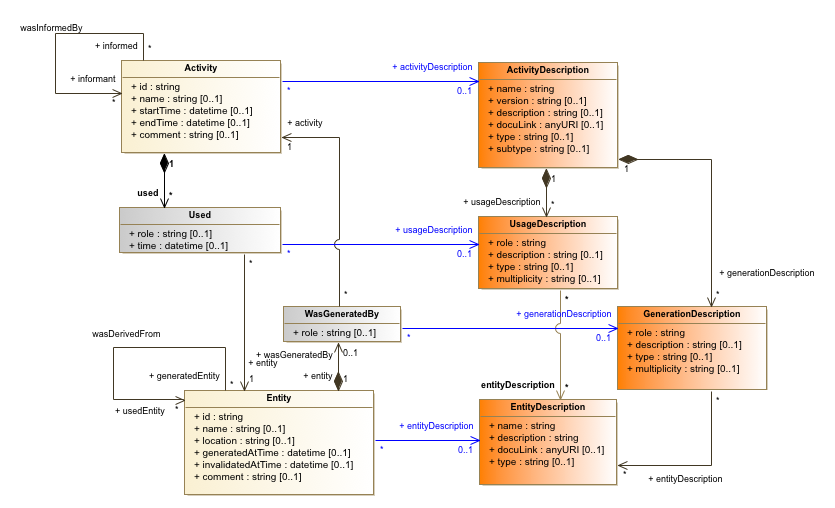
\includegraphics[width=1.0\textwidth]{PROV_Fig5.png}
\caption[Partial class diagram focused on description classes.]{Partial class diagram focused on description classes.}
\label{fig:classdiagram_descriptions}
\end{figure}


\subsubsection{ActivityDescription class}
\label{sec:activity_desc}


\begin{table}[ht]
\small
\tymax  0.5\textwidth
\textbf{\normalsize ActivityDescription}\vspace{0.25em}\\
\begin{tabulary}{1.0\textwidth}{llL}
\toprule
\head{Attribute} &  \head{Data type} & \head{Description}\\
\midrule
\textbf{name}         & string & a human-readable name\\
version      & string & a version number, if applicable (e.g., for the code used)\\
description  & string & additional free text describing how the activity works internally\\
docurl       & anyURI & link to further documentation on this activity, e.g., a
paper, the source code in a version control system etc.\\
type        & string & type of the activity\\
subtype     & string & more specific subtype of the activity\\
\bottomrule
\end{tabulary}
\caption[Attributes of the \class{ActivityDescription} class]{Attributes of the \class{ActivityDescription} class. Attributes in \textbf{bold} are mandatory and must not be null.
}\label{tab:activitydescription}
\end{table}


The information necessary to describe how an activity works internally are stored in \class{ActivityDescription} objects.

\class{ActivityDescription} is directly attached to \class{Activity} and can thus be seen as a list of attributes that can be known before an \class{Activity} instance is created.

There must be exactly zero or one \class{ActivityDescription} instance per activity.
If an activity is linked to an \class{ActivityDescription} instance, \class{Used}/\class{WasGeneratedBy}/\class{Entity} objects bound to this activity must refer to the description elements composing the \class{ActivityDescription}.

The activity \attribute{type} is a free text attribute, but if one of the terms in Table \ref{tab:activitydescription-types} applies, it should be used.
The activity \attribute{subtype} is a free text attribute to be used internally by the project that defined \class{ActivityDescription} instances (e.g., mosaicing, denoising, photometric calibration, cross correlation).


\begin{table}[ht]
\small
\tymax  0.5\textwidth
\textbf{\normalsize ActivityDescription types}\vspace{0.25em}\\
\begin{tabulary}{1.0\textwidth}{lp{8cm}}
\toprule
\head{Type} & \head{Description} \\
\midrule
Observation    & active acquisition of information on a phenomenon\\
Simulation     & generation of data through a computational process\\
Reduction      & transformation of digital information into a corrected, ordered, and simplified form\\
Calibration    & transformation and comparison of measurement values with respect to a calibration standard of known accuracy\\
Reconstruction & estimation of physical properties using indirect information\\
Selection      & application of filters or criteria to select partial information\\
Analysis       & process of inspecting, cleaning, transforming, and modeling data with the goal of discovering useful information, informing conclusions, and supporting decision-making\\
\bottomrule
\end{tabulary}
\caption[Terms applicable as activity types.]{Terms applicable as activity types.}
\label{tab:activitydescription-types}
\end{table}



\subsubsection{EntityDescription class}
\label{sec:entity_desc}


\begin{table}[ht]
\small
\tymax  0.5\textwidth
\textbf{\normalsize EntityDescription}\vspace{0.25em}\\
\begin{tabulary}{\textwidth}{llL}
\toprule
\head{Attribute} & \head{Data type} & \head{Description}\\
\midrule
\textbf{name}       & string & a human-readable name for the entity description\\
description  & string & a descriptive text for this kind of entity\\
docurl   & anyURI & link to more documentation\\
type      & string & type of the entity\\
\bottomrule
\end{tabulary}
\caption[Attributes of the \class{EntityDescription} class]{Attributes of the \class{EntityDescription} class. Attributes in \textbf{bold} are mandatory and must not be null.
}\label{tab:entitydescription}
\end{table}


The \class{EntityDescription} class is meant to store descriptive information for different categories of entities. It contains information that is known before an \class{Entity} instance is created. The \class{EntityDescription} general attributes are summarized in Table~\ref{tab:entitydescription}.

For example, a specific category of entities in a project may be defined in details in a document or on a webpage (e.g., a CTA DL3 file, a CCD device, a photographic plate).

The entity \attribute{type} is a free text attribute, that contains the general category of the entity, e.g., if it is data, a document, a vizualization, a device.

The \class{EntityDescription} class should not contain information about the usage of the data, in particular, it generally tells nothing about them being used as input or generated as output. This kind of information should be provided by the relations (and their descriptions) between activities and entities (see Sections~\ref{sec:entity-activity-relations} and \ref{sec:use_gen_desc}).


\subsubsection{UsageDescription and GenerationDescription classes}
\label{sec:use_gen_desc}

\begin{table}[h!]
\small
\tymax  0.5\textwidth
\textbf{\normalsize UsageDescription}\vspace{0.25em}\\
\begin{tabulary}{1.0\textwidth}{llL}
\toprule
\head{Attribute} &  \head{Data type} & \head{Description}\\
\midrule
\textbf{role} & string   & function of the entity with respect to the activity \\
description  & string & a descriptive text for this kind of usage \\
type    & string   & type of relation, see Section~\ref{sec:ugtypes} \\
multiplicity & string & Number of expected input entities to be used with the given role. The multiplicity syntax is similar to that of VO-DML (\citealt{2018ivoa.spec.0910L}, \S4.19) in the form `minOccurs..maxOccurs'' or a single value if minOccurs and maxOccurs are identical, e.g., ``1'' for one item, ``*'' for unbounded or ``3..*'' for unbounded with at least 3 items. \\
\bottomrule
\end{tabulary}
\caption[Attributes of the \class{UsageDescription} class]{Attributes of the \class{UsageDescription} class. Attributes in \textbf{bold} are mandatory and must not be null.}
\label{tab:usagedescription}
\end{table}


\begin{table}[h!]
\small
\tymax  0.5\textwidth
\textbf{\normalsize GenerationDescription}\vspace{0.25em}\\
\begin{tabulary}{1.0\textwidth}{llL}
\toprule
\head{Attribute} & \head{Data type} & \head{Description}\\
\midrule
\textbf{role} & string & function of the entity with respect to the activity \\
description  & string & a descriptive text for this kind of generation \\
type & string   & type of relation, see section \ref{sec:ugtypes} \\
multiplicity & string & Number of expected output entities that will be generated with the given role. The multiplicity syntax is similar to that of VO-DML (\citealt{2018ivoa.spec.0910L}, \S4.19) in the form `minOccurs..maxOccurs'' or a single value if minOccurs and maxOccurs are identical, e.g., ``1'' for one item, ``*'' for unbounded or ``3..*'' for unbounded with at least 3 items. \\
\bottomrule
\end{tabulary}
\caption[Attributes of the \class{GenerationDescription} class]{Attributes of the \class{GenerationDescription} class. Attributes in \textbf{bold} are mandatory and must not be null.}
\label{tab:wasgeneratedbydescription}
\end{table}


In order to describe more precisely an activity, the expected inputs and outputs of this activity should be specified.

We introduce the \class{UsageDescription} and the \class{GenerationDescription} classes, that are meant to store the information about the usage or generation of entities that is known before an activity instance is executed, i.e.~what we expect to store in the \class{Used} and \class{WasGeneratedBy} relations (see \ref{sec:entity-activity-relations}).
Instances of \class{Used} (respectively \class{WasGeneratedBy}) may thus point to an instance of \class{UsageDescription} (respectively \class{GenerationDescription}).

If a \class{UsageDescription} (respectively \class{GenerationDescription}) instance is defined, the \attribute{role} attribute of the related \class{Used} (respectively \class{WasGeneratedBy}) instances must match the \attribute{role} attribute of this \class{UsageDescription} (respectively \class{GenerationDescription}) instance.

A \attribute{multiplicity} attribute should be specified to indicate the number of entities expected to share the same role for a given \class{ActivityDescription} instance, e.g., in the case of the stacking of images, several images are expected with the same input role (\attribute{multiplicity=*}).

When related to the \class{UsageDescription} or \class{GenerationDescription}, the attributes of \class{EntityDescription} (see Section~\ref{sec:entity_desc}) help to describe the category of entities expected as an input or an output in an activity.
For example: if the input bias files are expected to be in FITS format, the \class{UsageDescription} object would have a relation to a \class{DatasetDescription} object with \attribute{contentType}=`application/fits'' (see Section~\ref{sec:dataset_entity} for this specific type of entity).


\subsubsection{Types of Usage and Generation}
\label{sec:ugtypes}

The typing of those relations is particularly needed to enable quality assessment and identification of error sources in the process (see goals C and D in Section \ref{sec:goals}), so as to facilitate the exploration of provenance information. 

The type of usage or generation is a free text attribute, but if one of the terms in Table \ref{tab:usage-generation-types} applies, it should be used.

\begin{table}[ht]
\small
\tymax  0.5\textwidth
\begin{tabulary}{1.0\textwidth}{Lp{8cm}}
\toprule
\head{Type} & \head{Description} \\
\midrule
Main           & main input or output entities of the activity, i.e.~strictly necessary, and the primary objective of the activity\\
Calibration    & usage of an entity to calibrate another entity\\
Preview        & generation of a quick representation of an entity\\
Setup          & usage of an entity as configuration information, see also Section~\ref{sec:configurationpackage}\\
Quality        & generation of information that helps to assess the quality of the activity results, e.g., errors, warnings, flags, percentage of overexposed pixels\\
Log            & generation of logging information\\
Context        & contextual information that influences the activity, but for which there are no or little control at the moment of its execution, examples: temperature, wind, conditions of observation, execution platform, operating system, instrumental context\\
\bottomrule
\end{tabulary}
\caption[Terms applicable as usage or generation type.]{Terms applicable as usage or generation type.}
\label{tab:usage-generation-types}
\end{table}

The type ``Main'' indicates the main input and output entities of an activity. It should help to provide the minimum relevant data flow to the initial entity or activity, i.e.~to find the most relevant progenitors.


\subsection{Specific types of Entity classes}
\label{sec:spec_entities}

\class{Entity} and \class{EntityDescription} classes carry the minimum metadata that can apply to any kind of entity without specifying the nature or the structure of the content of the entity. 
In some cases, the structure of the content is relevant information to assess the usefulness of the entity, in particular for datasets.
In some other cases, the content itself of an entity is relevant information to assess the usefulness of the related entities or activities. Such content must then be exposed as properly described values.

In astronomy and the VO, we thus define two main types of entity classes:

\begin{itemize}
    \item \textbf{Dataset}: a dataset is a resource which encodes data in a defined structure. It is generally a file or a set of files which are considered to be a single deliverable. The content may be e.g., a cube, an image, a table, a list.
    \item \textbf{Value}: a value is an atomic piece of data with a given value type (e.g., a data type such as boolean, integer, real, string).
\end{itemize}

\begin{figure}[ht]
\centering
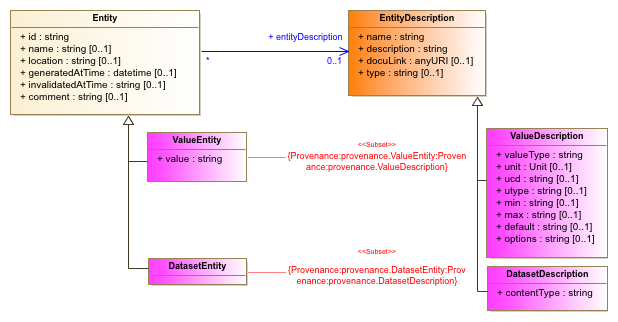
\includegraphics[width=1.0\textwidth]{PROV_Fig6.png}
\caption[Partial class diagram focused on specific types of \class{Entity} classes.]{Partial class diagram focused on Specific types of \class{Entity} classes.}
\label{fig:classdiagram_entityclasses}
\end{figure}

As shown in Figure~\ref{fig:classdiagram_entityclasses}, the entity description classes for both \class{ValueEntity} and \class{DatasetEntity} are subsetted respectively as \class{ValueDescription} and \class{DatasetDescription}.

We anticipate that more specific categories of entities can be defined by the projects (for example, a device, a document, a vizualization). The \attribute{type} attribute of the \class{EntityDescription} class should be used to differentiate the different categories of entities.


\subsubsection{DatasetEntity and DatasetDescription classes}
\label{sec:dataset_entity}

The handling of datasets is implemented in the model by a \class{DatasetEntity} class. A corresponding \class{DatasetDescription} class contains a \attribute{contentType} attribute that must not be null (see Table~\ref{tab:datasetdescription}).

The \attribute{contentType} indicates the MIME-type or format of a dataset, or a more precise structure, following the definition of the attribute \attribute{access\_format} defined in ObsCoreDM (\citet{2017ivoa.spec.0509L}, Section 4.7).

\begin{table}[ht]
\small
\tymax  0.5\textwidth
\textbf{\normalsize DatasetDescription}\vspace{0.25em}\\
\begin{tabulary}{1.0\textwidth}{llL}
\toprule
\head{Attribute} &  \head{Data type} & \head{Description}\\
\midrule
\textbf{contentType}  & string  & format of the dataset, MIME type when applicable \\
\bottomrule
\end{tabulary}
\caption[Attributes of the \class{DatasetDescription} class]{Attributes of the  \class{DatasetDescription} class. The class also inherits the attributes of \class{EntityDescription} listed in Table \ref{tab:entitydescription}. Attributes in \textbf{bold} are mandatory and must not be null.}
\label{tab:datasetdescription}
\end{table}


\subsubsection{ValueEntity and ValueDescription classes}

The handling of values is implemented in the model by a \class{ValueEntity} class that contains a \attribute{value} attribute. A corresponding \class{ValueDescription} class contains attributes commonly used in the VO to qualify values. Those attributes are listed in Table~\ref{tab:valuedescription}.

\begin{table}[ht]
\small
\tymax  0.5\textwidth
\textbf{\normalsize ValueEntity}\vspace{0.25em}\\
\begin{tabulary}{1.0\textwidth}{llL}
\toprule
\head{Attribute} &  \head{Data type} & \head{Description}\\
\midrule
\textbf{value}  & string  & the value of the entity. If a corresponding \class{ValueDescription}.\attribute{valueType} attribute is set, the value string can be interpreted by this \attribute{valueType}. \\
\bottomrule
\end{tabulary}
\caption[Attributes of the \class{ValueEntity} class]{Attributes of the  \class{ValueEntity} class. The class also inherits the attributes of \class{EntityDescription} listed in Table \ref{tab:entitydescription}. Attributes in \textbf{bold} are mandatory and must not be null.}
\label{tab:valueentity}
\end{table}

\begin{table}[ht]
\small
\tymax  0.5\textwidth
\textbf{\normalsize ValueDescription}\vspace{0.25em}\\
\begin{tabulary}{1.0\textwidth}{p{2cm}LL}
\toprule
\head{Attribute} &  \head{Data type} & \head{Description}\\
\midrule
\textbf{valueType} & VotableFieldFormat & description of a value from a combination of \attribute{datatype}, \attribute{arraysize} and \attribute{xtype} following VOTable 1.3 \citep[][, \S4.1]{2013ivoa.spec.0920O} \\
unit        & Unit & VO unit, see \ref{sect:Units} and \citet{2014ivoa.spec.0523D} for recommended unit representation \\
ucd         & string  & Unified Content Descriptor, supplying a standardized classification of the physical quantity, see \citet{2018ivoa.spec.0527M}\\
utype       & string  & Utype, meant to express the role of the value in the context of an external data model, see \citet{note:utypeusage} \\
\bottomrule
\end{tabulary}
\caption[Attributes of the \class{ValueDescription} class]{Attributes of the \class{ValueDescription} class. The class also inherits the attributes of \class{EntityDescription} listed in Table \ref{tab:entitydescription}. Attributes in \textbf{bold} are mandatory and must not be null.}
\label{tab:valuedescription}
\end{table}



\subsection{Activity configuration}
\label{sec:configuration}

Configuring an activity is the way to set parameters so that the activity occurs in the desired conditions.

In some cases developed in Section~\ref{sec:goals} (goals C and D in particular), configuration information is relevant to assess the quality and reliability of an activity or an entity, and to identify the location of configuration errors in a processing. It also facilitates the re-execution of an activity (reproducibility).

Configuration information may be carried by entities using the core features, where an entity (e.g., \class{ValueEntity} and \class{DatasetEntity} instances) is referenced in \class{Used} relations with a given \attribute{role} and \attribute{type}=“Setup”. With this solution, the configuration information is independent from the activity and can be generated and used as any entity.

The data model also provides a specialized \class{ActivityConfiguration} package to directly attach configuration information to an activity. This package is composed of a \class{WasConfiguredBy} relation connecting  \class{Parameter} and \class{ConfigFile} classes with the \class{Activity} class (see~\ref{sec:configurationpackage}). With this solution the configuration information is independent from the entities, and seen as part of the activity.


\begin{figure}[hbt]
\centering
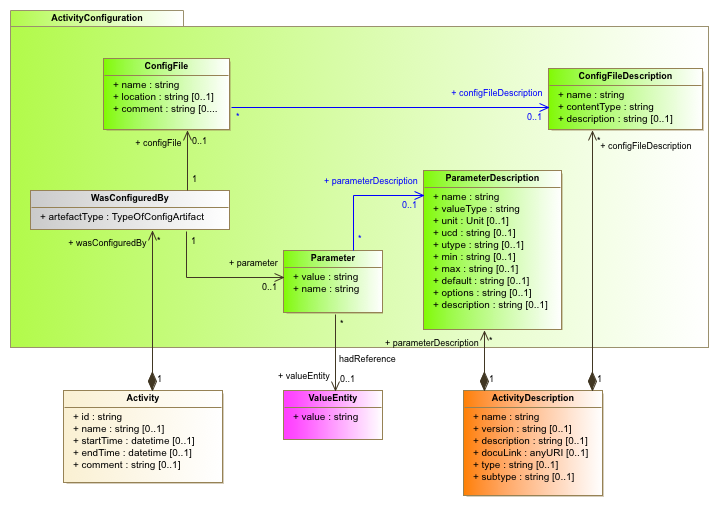
\includegraphics[width=1.0\textwidth]{PROV_Fig7.png}
% Mireille: updated the diagram file for the last version with the proper cardinalities for Parameter and ConfigFile
\caption[Partial class diagram focused on the \class{ActivityConfiguration} package.]{Partial class diagram focused on the \class{ActivityConfiguration} package. The \class{Parameter} and \class{ConfigFile} classes provide configuration information for an \class{Activity} instance. The right side of the diagram shows the descriptions, where an \class{ActivityDescription} class is bound with the \class{ParameterDescription} and \class{ConfigFileDescription} classes.}
\label{fig:activityconfig}
\end{figure}


\subsubsection{Overview of the ActivityConfiguration package} \label{sec:configurationpackage}

As shown in Figure \ref{fig:activityconfig} the \class{ActivityConfiguration} package contains two classes for the execution side: \class{Parameter} and \class{ConfigFile} which are connected to an \class{Activity} instance via the \class{WasConfiguredBy} association class.
An \class{Activity} may thus be configured by a set of \class{Parameter} instances, by \class{ConfigFile} instances, or by a combination of both.

The corresponding description classes, \class{ParameterDescription} and \class{ConfigFileDescription}, are both defined in the context of the description of an activity.
There can be several instances of a \class{Parameter} (respectively \class{ConfigFile}) that are described by the same instance of \class{ParameterDescription} (respectively \class{ConfigFileDescription}).


\subsubsection{Parameter and ParameterDescription classes}
\label{sec:parameterandD}

\begin{table}[h!]
\small
\tymax  0.5\textwidth
 \textbf{\normalsize Parameter}\vspace{0.25em}\\
 \begin{tabulary}{1.0\textwidth}{llL}
 \toprule
 \head{Attribute} & \head{Data type}   & \head{Description}\\
 \midrule
\textbf{name}  & string & name of the parameter \\
\textbf{value} & string & the value of the parameter. If a corresponding \class{ParameterDescription}.\attribute{valueType} attribute is set, the value string can be interpreted by this \attribute{valueType}. \\
\bottomrule
\end{tabulary}
\caption[Attributes of the \class{Parameter} class]{Attributes of the \class{Parameter} class. Attributes in \textbf{bold} are mandatory and must not be null.}
\label{tab:param}
\end{table}

\begin{table}[h!]
\small
\tymax  0.5\textwidth
\textbf{\normalsize ParameterDescription}\vspace{0.25em}\\
\begin{tabulary}{1.0\textwidth}{lLL}
 \toprule
 \head{Attribute} & \head{Data type}   & \head{Description}\\
 \midrule
\textbf{name} & string & name of the parameter \\
\textbf{valueType} & VotableFieldFormat & description of a value from a combination of \attribute{datatype}, \attribute{arraysize} and \attribute{xtype} following VOTable 1.3 \citep[][, \S4.1]{2013ivoa.spec.0920O} \\
description & string  & a descriptive text for the parameter \\
unit        & Unit  & VO unit, see \ref{sect:Units} and \citet{2014ivoa.spec.0523D} for recommended unit representation \\
ucd         & string  & Unified Content Descriptor, supplying a standardized classification of the physical quantity, see \citet{2018ivoa.spec.0527M} \\
utype       & string  & Utype, meant to express the role of the parameter in the context of an external data model, see \citet{note:utypeusage} \\
min         & string & minimum value as a string whose value can be interpreted by the \attribute{valueType} attribute \\
max         & string & maximum value as a string whose value can be interpreted by the \attribute{valueType} attribute\\
options     & array of strings & array of possible values\\
default     & string & the default value of the parameter as a string whose value can be interpreted by the \attribute{valueType} attribute \\
\bottomrule
\end{tabulary}
\caption[Attributes of the \class{ParameterDescription} class]{Attributes of the  \class{ParameterDescription} class. Attributes in \textbf{bold} are mandatory and must not be null.}
\label{tab:Paramdescription}
\end{table}

The \class{Parameter} class contains a \attribute{value} and a \attribute{name} attribute that must be set (Table~\ref{tab:param}).

The \class{ParameterDescription} class describes the parameter \attribute{value} attribute similarly to the \class{ValueEntity} and \class{ValueDescription} classes. Those attributes are listed in Table~\ref{tab:Paramdescription}.

If a \class{ParameterDescription} instance is defined, the \attribute{name} attribute of the related \class{Parameter} instances must match the \attribute{name} attribute of this \class{ParameterDescription} instance.

The \class{Parameter} instance may refer to a \class{ValueEntity} instance using a \textit{hadReference} relation which gives the origin of the parameter value.


\subsubsection{ConfigFile and ConfigFileDescription classes}

\begin{table}[ht]
\small
\tymax  0.5\textwidth
 \textbf{\normalsize ConfigFile}\vspace{0.25em}\\
 \begin{tabulary}{1.0\textwidth}{llL}
 \toprule
 \head{Attribute} & \head{Data type}   & \head{Description}\\
 \midrule
\textbf{name} &  string & a human-readable name for the config file \\
\textbf{location} & string  &  a path to the config file, e.g., a URL/URI \\
comment & string  & text containing comments on the config file  \\
\bottomrule
\end{tabulary}
\caption[Attributes of the \class{ConfigFile} class]{Attributes of the \class{ConfigFile} class. Attributes in \textbf{bold} are mandatory and must not be null.}
\label{tab:configfile}
\end{table}

\begin{table}[ht]
\small
\tymax  0.5\textwidth
\textbf{\normalsize ConfigFileDescription}\vspace{0.25em}\\
\begin{tabulary}{1.0\textwidth}{llL}
 \toprule
 \head{Attribute} & \head{Data type}   & \head{Description}\\
 \midrule
\textbf{name}    & string & a human-readable name for the config file \\
\textbf{contentType}  & string  & format of the config file, MIME type when applicable \\
description     & string  & a descriptive text for the config file \\
\bottomrule
\end{tabulary}
\caption[Attributes of the \class{ConfigFileDescription} class]{Attributes of the  \class{ConfigFileDescription} class. Attributes in \textbf{bold} are mandatory and must not be null.}
\label{tab:configfiledescription}
\end{table}

The \class{ConfigFile} points to a structured, machine readable file, where parameters for running an activity are stored. It contains a \attribute{location} and a \attribute{name} that must be set, and a \attribute{comment} attribute (Table~\ref{tab:configfile}).

The \class{ConfigFileDescription} class indicates the format in which the content of the file is provided using a \attribute{contentType} attribute (see Table~\ref{tab:configfiledescription}).

If a \class{ConfigFileDescription} instance is defined, the \attribute{name} attribute of the related \class{ConfigFile} instances must match the \attribute{name} attribute of this \class{ConfigFileDescription} instance.


\subsubsection{Relations with Activity class}

\begin{table}[ht]
\small
\tymax  0.5\textwidth
 \textbf{\normalsize WasConfiguredBy}\vspace{0.25em}\\
 \begin{tabulary}{1.0\textwidth}{llL}
 \toprule
 \head{Attribute} & \head{Data type}   & \head{Description}\\
 \midrule
\textbf{artefactType} &  TypeOfConfigArtefact & literal that takes the value ``Parameter'' or ``ConfigFile'' to indicate the type of class pointed by the \class{WasConfiguredBy} instance. \\
\bottomrule
\end{tabulary}
\caption[Attributes of the \class{WasConfiguredBy} class]{Attributes of the \class{WasConfiguredBy} class. Attributes in \textbf{bold} are mandatory and must not be null.}
\label{tab:WasConfiguredBy}
\end{table}

The relation of \class{Parameter} and \class{ConfigFile} to \class{Activity} is formalized by a \class{WasConfiguredBy} class. There must be exactly one instance connected to a \class{WasConfiguredBy} instance, either a \class{Parameter} instance or a \class{ConfigFile} instance. The \class{WasConfiguredBy} class contains the attribute \attribute{artefactType} to indicate the type of class pointed by the \class{WasConfiguredBy} instance (see Table~\ref{tab:WasConfiguredBy}).

The life cycle of a \class{Parameter} instance (or \class{ConfigFile} instance) is the one of the corresponding \class{Activity} instance.
The life cycle of a \class{ParameterDescription} instance (or \class{ConfigFileDescription} instance) is the one of the corresponding \class{ActivityDescription} instance.
This means that when an activity is deleted from the provenance repository, its parameters and config files also disappear.

Several activities launched with various possible values for a parameter share the same \class{ParameterDescription} instance.
For instance, a cube analysis activity with a parameter ``nbofChannels'' will point to the corresponding instance of \class{ParameterDescription} (\attribute{name} = ``nbofChannels'', \attribute{ucd} = ``meta.number'', \attribute{unit} = Null, \attribute{description} = ``Nb of channel used for segmentation'').
`
Similarly, we can foresee a number of different \class{ConfigFile} instances used for various instances of an \class{Activity}, which rely on the same \class{ConfigFileDescription} instance bound to the corresponding \class{ActivityDescription} instance.
